% Relatorio da Versao 2 -- formatacao reproduzindo o modelo de artigos da SBC
% (A4; margens 3,5/2,5/3/3 cm; Times 12; titulo 16 pt; secoes 13 pt; resumo recuado 0,8 cm).
\documentclass[12pt,a4paper]{article}
\usepackage[utf8]{inputenc}
\usepackage[T1]{fontenc}
\usepackage{mathptmx}
\usepackage[a4paper,top=3.5cm,bottom=2.5cm,left=3cm,right=3cm]{geometry}
\usepackage{graphicx,booktabs,tabularx,array,float,url,microtype,indentfirst}
\usepackage{amsmath}
\usepackage[font=small,labelfont=bf,textfont=bf,labelsep=period]{caption}
\usepackage{subcaption}
\usepackage{titlesec}
\usepackage{enumitem}
\usepackage{xcolor}
\usepackage{tikz}
\usetikzlibrary{arrows.meta,positioning,fit,calc}
\usepackage[hidelinks]{hyperref}

% Termos em portugues (sem pacote babel de portugues no ambiente)
\renewcommand{\figurename}{Figura}
\renewcommand{\tablename}{Tabela}
\renewcommand{\refname}{Referências}

% Paragrafos no estilo SBC: recuo de 1,27 cm e 6 pt depois
\setlength{\parindent}{1.27cm}
\setlength{\parskip}{6pt}
\titleformat{\section}{\fontsize{13}{15}\bfseries}{\thesection.}{0.5em}{}
\titlespacing*{\section}{0pt}{12pt}{6pt}
\titleformat{\subsection}{\normalsize\bfseries}{\thesubsection.}{0.5em}{}
\titlespacing*{\subsection}{0pt}{12pt}{6pt}
\setlist{nosep,leftmargin=1.27cm}
\urlstyle{same}
\sloppy

\newenvironment{resumo}[1]%
  {\par\vspace{6pt}\noindent\begin{list}{}{\setlength{\leftmargin}{0.8cm}\setlength{\rightmargin}{0.8cm}}%
   \item[]\textbf{#1.}\itshape\ }%
  {\end{list}}

\begin{document}

\begin{center}
{\fontsize{16}{19}\selectfont\bfseries Servidor HTTP com Qualidade de Serviço em C e Pthreads:\\
controle de taxa por IP, admissão e estimativa de RTT (Versão~2)\par}
\vspace{12pt}
{\bfseries Rodrigo Silveira, João Gabriel Oliveira da Silva, Nicolas Ramos\par}
\vspace{6pt}
Curso de Engenharia de Computação -- Universidade Federal do Pampa (UNIPAMPA)\\
Campus Bagé -- Bagé, RS -- Brasil\par
\vspace{4pt}
Fundamentos e Avaliação de Redes de Computadores -- 2026/2 -- Relatório da segunda versão\par
\end{center}

\begin{resumo}{Abstract}
This report presents the second version of an HTTP/1.1 server written in C with POSIX
threads. Building on the first version (concurrent clients and persistent connections),
it adds Quality of Service mechanisms: per-source-IP rate control for every object except
HTML, with the rate of an address shared among its simultaneous connections through a
per-IP virtual clock; admission control bounded by the server's maximum throughput
(HTTP 503); and per-client estimates of round-trip time, end-to-end delay and bandwidth,
obtained from an HTML request followed by the request for its first object and shown in a
real-time panel. Experiments over loopback with distinct source addresses show measured
rates within 0.7\% of the configured values, a fair split among three connections of the
same address, and correct admission decisions. We also show that Nagle's algorithm combined
with delayed acknowledgments inflated the measured RTT from under 1~ms to about 41~ms, and
how disabling it fixed the measurement.
\end{resumo}

\begin{resumo}{Resumo}
Este relatório apresenta a segunda versão de um servidor HTTP/1.1 escrito em C com
Pthreads. Partindo da primeira versão (clientes concorrentes e conexões persistentes), ela
acrescenta mecanismos de Qualidade de Serviço: controle de taxa por IP de origem para todos
os objetos, exceto o HTML, com a taxa de um endereço dividida entre as suas conexões
simultâneas por meio de um relógio virtual por IP; controle de admissão limitado pela vazão
máxima do servidor (HTTP 503); e estimativas, por cliente, de RTT, atraso fim-a-fim e
largura de banda, obtidas a partir da requisição do HTML seguida da requisição do seu
primeiro objeto e exibidas em um painel em tempo real. Experimentos em loopback, com
endereços de origem distintos, mostram taxas medidas a menos de 0,7\% das configuradas,
divisão justa entre três conexões do mesmo endereço e decisões de admissão corretas.
Mostra-se também que o algoritmo de Nagle, combinado com o ACK atrasado, inflava o RTT
medido de menos de 1~ms para cerca de 41~ms, e como desativá-lo corrigiu a medida.
\end{resumo}

\section{Introdução}

Aplicações diferentes impõem requisitos distintos de qualidade de serviço (QoS) à rede:
algumas toleram atraso, outras dependem de vazão garantida
[Kurose e Ross 2013; Forouzan 2013]. Do lado do servidor, uma forma simples de oferecer
tratamento diferenciado é controlar a taxa com que cada cliente é atendido e recusar
novos clientes quando a capacidade contratada se esgota.

O trabalho prático da disciplina pede um servidor HTTP em linguagem C com Pthreads,
desenvolvido em versões incrementais. A primeira versão, já entregue, atende vários
clientes simultaneamente e segue o HTTP/1.1 com conexões persistentes
[Fielding et al. 2022b]. Esta segunda versão acrescenta os mecanismos de QoS previstos
na especificação: (i)~envio dos objetos, exceto o arquivo HTML, com taxa controlada
conforme o IP de origem, lida de um arquivo auxiliar, e 1000~kbps para IPs não cadastrados,
se viável; (ii)~divisão da taxa entre conexões simultâneas do mesmo IP; (iii)~controle de
admissão que não permita exceder a vazão máxima do servidor, informada como parâmetro; e
(iv)~apresentação em tempo real dos clientes atendidos, com estimativas de atraso
fim-a-fim e largura de banda baseadas no RTT.

A Seção~\ref{sec:desenv} descreve a arquitetura e os algoritmos, a
Seção~\ref{sec:aval} apresenta a avaliação experimental e a Seção~\ref{sec:concl}
conclui. O código está em \url{https://github.com/nicolasURamos/t1-redes}.

\section{Desenvolvimento}\label{sec:desenv}

\subsection{Arquitetura}

O servidor mantém o modelo da primeira versão: uma thread destacada por conexão, que trata
todas as requisições daquela conexão até um \texttt{Connection: close}, um erro ou 15~s de
inatividade. A versão~2 introduz dois módulos novos (Tabela~\ref{tab:modulos}) e liga-os
ao código existente em poucos pontos. A Figura~\ref{fig:arq} mostra o caminho de uma conexão.

\begin{table}[H]
\centering
\caption{Organização do código (módulos novos da versão 2 em destaque).}
\label{tab:modulos}
\small
\begin{tabularx}{\linewidth}{@{}lX@{}}
\toprule
Arquivo & Responsabilidade \\
\midrule
\texttt{servidor.c} & Parâmetros, \textit{socket}, \texttt{accept}, \textit{timeouts}, \texttt{TCP\_NODELAY}; uma thread por conexão, que pede admissão ao iniciar \\
\texttt{http.c} & Leitura incremental, validação, laço \textit{keep-alive}; registra o instante de cada requisição \\
\texttt{arquivos.c} & Caminho seguro, MIME, envio em blocos; aplica o ritmo do IP (exceto HTML) \\
\textbf{\texttt{qos.c}} & Tabela de taxas, tabela de IPs ativos, admissão, relógio virtual por IP, medidas de RTT \\
\textbf{\texttt{painel.c}} & Thread que redesenha o painel a cada 1~s \\
\bottomrule
\end{tabularx}
\end{table}

\begin{figure}[H]
\centering
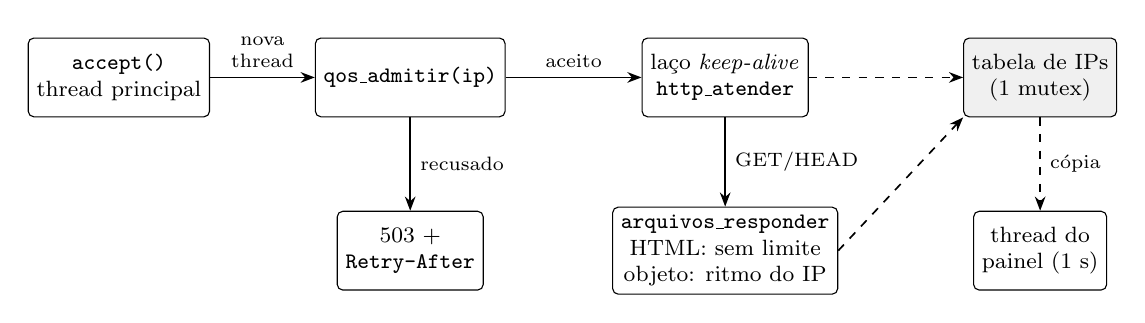
\begin{tikzpicture}[
  font=\footnotesize,
  box/.style={draw, rounded corners=2pt, align=center, minimum height=1.0cm, inner sep=3pt},
  arr/.style={-{Stealth[length=1.8mm]}, semithick},
  lbl/.style={font=\scriptsize, align=center}]
\node[box] (acc) at (0,0) {\texttt{accept()}\\thread principal};
\node[box] (adm) at (3.7,0) {\texttt{qos\_admitir(ip)}};
\node[box] (http) at (7.7,0) {laço \textit{keep-alive}\\\texttt{http\_atender}};
\node[box, fill=black!6] (tab) at (11.7,0) {tabela de IPs\\(1 mutex)};
\node[box] (rec) at (3.7,-2.2) {503 +\\\texttt{Retry-After}};
\node[box] (arq) at (7.7,-2.2) {\texttt{arquivos\_responder}\\HTML: sem limite\\objeto: ritmo do IP};
\node[box] (pan) at (11.7,-2.2) {thread do\\painel (1 s)};
\draw[arr] (acc) -- node[lbl, above]{nova\\thread} (adm);
\draw[arr] (adm) -- node[lbl, above]{aceito} (http);
\draw[arr] (adm) -- node[lbl, right]{recusado} (rec);
\draw[arr] (http) -- node[lbl, right]{GET/HEAD} (arq);
\draw[arr, dashed] (http) -- (tab);
\draw[arr, dashed] (arq.east) -- (tab.south west);
\draw[arr, dashed] (tab) -- node[lbl, right]{cópia} (pan);
\end{tikzpicture}
\caption{Caminho de uma conexão na versão 2. Setas tracejadas indicam acesso ao estado compartilhado.}
\label{fig:arq}
\end{figure}

A execução recebe quatro parâmetros opcionais:
\texttt{./servidor [porta] [pasta] [vazao\_max\_kbps] [arquivo\_taxas]}.
O arquivo de taxas tem uma linha \texttt{IP taxa\_kbps} por endereço, admite comentários
com \texttt{\#} e gera aviso para linhas inválidas. IPs ausentes recebem 1000~kbps.

\subsection{Controle de taxa compartilhado por IP}

Cada IP com conexões ativas possui um registro com a sua taxa $R$ (kbps) e um relógio
virtual $T_{\mathrm{prox}}$, o instante a partir do qual o próximo bloco daquele IP pode
ser enviado. Antes de enviar um bloco de $n$ bytes de um objeto que não seja HTML, a
conexão executa, com o mutex travado:
\begin{equation}
t_{\mathrm{ini}} = \max\left(t_{\mathrm{agora}},\, T_{\mathrm{prox}}\right), \qquad
T_{\mathrm{prox}} \leftarrow t_{\mathrm{ini}} + \frac{8n}{1000\,R}\ \text{[s]}
\end{equation}
Em seguida, destrava o mutex, dorme até $t_{\mathrm{ini}}$ com
\texttt{clock\_nanosleep} em modo absoluto sobre \texttt{CLOCK\_MONOTONIC} e só então
envia o bloco. Como todas as conexões do mesmo IP reservam intervalos no mesmo relógio,
a soma das suas taxas nunca ultrapassa $R$ e a divisão entre elas sai automática,
inclusive quando conexões abrem ou fecham no meio de uma transferência. Essa abordagem
dispensa calcular $R/k$ para $k$ conexões, o que exigiria reajustar todas as conexões a
cada mudança de $k$. O termo $\max(\cdot)$ impede que um IP ocioso acumule crédito e
depois envie uma rajada, de modo semelhante a um balde de fichas de profundidade
mínima [Forouzan 2013].

O tamanho do bloco corresponde a cerca de 20~ms de dados na taxa do IP
($n = 1000R/8/50$ bytes), limitado entre 1460 e 65536 bytes. Blocos pequenos suavizam o
envio em taxas baixas; o limite inferior evita chamadas de sistema excessivas. O HTML é
enviado em blocos de 64~KiB e sem espera, como exige a especificação.

\subsection{Controle de admissão}

A admissão é decidida por endereço. Uma conexão de um IP que já tem conexões ativas é
sempre aceita e passa a dividir a taxa daquele IP. Um IP novo, de taxa $R$, só é aceito se
$C + R \le V_{\max}$, onde $C$ é a soma das taxas dos IPs ativos (vazão comprometida) e
$V_{\max}$ é a vazão máxima do servidor. Ao fechar a última conexão de um IP, a sua taxa é
subtraída de $C$. Assim, ``1000~kbps se viável'' significa que um IP não cadastrado só
entra se houver 1000~kbps livres.

O cliente recusado recebe \texttt{503 Service Unavailable} com
\texttt{Retry-After: 5} [Fielding et al. 2022a]. Fechar o \textit{socket} logo após
escrever o 503, com a requisição do cliente ainda não lida, faria o \textit{kernel} enviar
um RST, e o cliente poderia perder a resposta. Por isso o servidor fecha apenas o lado de
escrita (\texttt{shutdown}) e lê o que restar por até 1~s antes de fechar. Para que essa
espera nunca atrase o \texttt{accept}, a admissão é feita no início da thread de cada
conexão.

\subsection{Estimativa de RTT, atraso e largura de banda}

Seguindo a especificação, a estimativa usa duas requisições consecutivas do mesmo
cliente: a do HTML e a do primeiro objeto referenciado nele. Quando o servidor termina de
enviar um HTML, registra o instante da requisição ($t_{\mathrm{req,html}}$), o instante
do fim do envio ($t_{\mathrm{fim,html}}$) e o tamanho ($B$ bytes). Na chegada da
requisição seguinte de um objeto daquele IP ($t_{\mathrm{req,obj}}$), calcula:
\begin{equation}
\mathrm{RTT} = t_{\mathrm{req,obj}} - t_{\mathrm{fim,html}}, \qquad
\text{atraso} \approx \frac{\mathrm{RTT}}{2}, \qquad
\text{banda} = \frac{8B}{t_{\mathrm{req,obj}} - t_{\mathrm{req,html}}}
\end{equation}

O intervalo medido inclui o tempo que o cliente leva para processar o HTML; o atraso
RTT/2 é, portanto, uma estimativa superior. A banda é a vazão efetiva de um ciclo
completo, do pedido do HTML ao pedido do objeto; com HTML pequeno (694~bytes), ela é
dominada pelo RTT e subestima a capacidade do enlace. Como navegadores podem atrasar ou
paralelizar os pedidos de imagens, os experimentos usam \texttt{wget} e \texttt{curl},
como sugere a especificação. Cada medida também é registrada no log do servidor.

\subsection{Painel em tempo real}

Uma thread dedicada copia, a cada segundo, o estado da tabela de IPs (com o mutex travado
apenas durante a cópia) e imprime o painel: vazão máxima, comprometida e livre; e, por IP,
o número de conexões, a taxa configurada, a taxa real no último segundo, o RTT, o atraso e
a banda. Em terminal, a tela é redesenhada; redirecionado para arquivo, os quadros se
acumulam, o que permite registrar a evolução de um experimento.

\subsection{Processo de desenvolvimento e verificação}

O desenvolvimento seguiu etapas incrementais versionadas com Git: parâmetros e arquivo de
taxas; admissão; controle de taxa; medidas e painel; documentação e \textit{scripts} de
experimento. Cada etapa só avançou com compilação sem avisos
(\texttt{-Wall -Wextra -Wpedantic}) e com os testes automatizados passando. Aos seis
testes de integração da versão~1 foram somados seis testes de QoS, que usam endereços de
origem distintos no \textit{loopback} (127.0.0.1, .2 e .3), já que o Linux trata todo o
bloco 127.0.0.0/8 como local e o servidor enxerga cada endereço como um cliente diferente
(Tabela~\ref{tab:testes}). Uma execução dos testes com o ThreadSanitizer não apontou
condições de corrida no acesso ao estado compartilhado.

\begin{table}[H]
\centering
\caption{Testes automatizados de QoS (\texttt{make test}), com vazão máxima de 10000~kbps.}
\label{tab:testes}
\small
\begin{tabularx}{\linewidth}{@{}Xl@{}}
\toprule
Teste & Critério de aprovação \\
\midrule
HTML sem limite de taxa & $< 0{,}3$~s \\
1 download de 3{,}1~MB a 8000~kbps & entre 85\% e 125\% de 3{,}15~s \\
2 downloads simultâneos do mesmo IP & cada um entre 85\% e 125\% de 6{,}29~s \\
IP não cadastrado, 125~kB (1000~kbps) & entre 0{,}75 e 1{,}3~s \\
Admissão (8000 + 1000 ocupados, pedido de 4000) & 503 com \texttt{Retry-After}; aceito após liberar \\
RTT no painel após HTML + objeto & valor numérico $< 50$~ms \\
\bottomrule
\end{tabularx}
\end{table}

\textbf{Uso de inteligência artificial.} Conforme exigido pela especificação, registra-se
que o código e a documentação da versão~1 tiveram apoio do ChatGPT (OpenAI) e que a
implementação da versão~2 (\texttt{qos.c}, \texttt{painel.c}, alterações em
\texttt{servidor.c}, \texttt{http.c} e \texttt{arquivos.c}, testes de QoS e
\textit{script} de experimentos) teve apoio do Claude Code (Anthropic). O apoio está
indicado no comentário de topo de cada arquivo, no README e no histórico do repositório.
A equipe revisou, compilou e testou o código.

\section{Avaliação Experimental}\label{sec:aval}

\subsection{Ambiente e metodologia}

Os experimentos foram executados em um computador com Windows e WSL2 (Ubuntu 22.04,
GCC 11.4), com servidor e clientes na mesma máquina, pela interface de \textit{loopback}.
Para representar clientes distintos, o \textit{script} \texttt{scripts/experimentos.sh}
usa \texttt{curl -{}-interface} com os endereços de origem 127.0.0.1, 127.0.0.2 e 127.0.0.3.
O servidor foi iniciado com vazão máxima de 12000~kbps e com o arquivo de taxas do
repositório (127.0.0.1: 8000~kbps; 127.0.0.2: 4000~kbps; 127.0.0.3: 2000~kbps). O objeto
transferido é \texttt{imagem1.bmp}, de 3.145.782~bytes (25,17~Mbit). O tempo esperado de
uma transferência é o tamanho em bits dividido pela taxa da conexão, e a taxa medida é
calculada a partir da velocidade média informada pelo \texttt{curl}
(bytes/s $\times 8 / 1000$).

\subsection{Resultados}

A Tabela~\ref{tab:resultados} resume os cenários. Em todos, a taxa medida ficou a menos
de 0,7\% da taxa prevista. No cenário com três downloads simultâneos do mesmo IP, cada
conexão recebeu cerca de um terço dos 8000~kbps e a soma (8021~kbps) ficou dentro do
limite do endereço, o que confirma a divisão da taxa. No cenário com dois IPs, cada
endereço recebeu a sua própria taxa ao mesmo tempo, sem interferência mútua. O desvio
positivo, da ordem de 0,15\%, vem do primeiro bloco de cada transferência, enviado sem
espera, já que o relógio do IP ainda está no passado.

\begin{table}[H]
\centering
\caption{Resultados dos experimentos (vazão máxima de 12000~kbps; objeto de 25,17~Mbit). O desvio é da taxa medida; na última linha, do tempo total.}
\label{tab:resultados}
\small
\setlength{\tabcolsep}{4pt}
\begin{tabularx}{\linewidth}{@{}Xrrrrr@{}}
\toprule
Cenário & Taxa & Tempo & Tempo & Taxa & Desvio \\
 & prevista & previsto & medido & medida & \\
 & (kbps) & (s) & (s) & (kbps) & \\
\midrule
1 download, 127.0.0.1 & 8000 & 3,146 & 3,141 & 8012 & +0,15\% \\
3 simultâneos, 127.0.0.1 (conexão 1) & 2667 & 9,437 & 9,426 & 2670 & +0,12\% \\
3 simultâneos, 127.0.0.1 (conexão 2) & 2667 & 9,437 & 9,381 & 2683 & +0,61\% \\
3 simultâneos, 127.0.0.1 (conexão 3) & 2667 & 9,437 & 9,431 & 2668 & +0,05\% \\
2 IPs juntos: 127.0.0.1 & 8000 & 3,146 & 3,141 & 8012 & +0,15\% \\
2 IPs juntos: 127.0.0.2 & 4000 & 6,292 & 6,281 & 4007 & +0,17\% \\
\texttt{wget -p} (HTML + 3 imagens) & 8000 & 9,437 & 9,46 & -- & +0,24\% \\
\bottomrule
\end{tabularx}
\end{table}

\textbf{Admissão.} Com 127.0.0.1 (8000~kbps) e 127.0.0.3 (2000~kbps) baixando, a vazão
comprometida era de 10000~kbps. Um pedido de 127.0.0.2, de 4000~kbps, exigiria
14000~kbps e recebeu 503, como registrado pelo cliente e pelo log do servidor
(``Recusado (vazao maxima atingida): 127.0.0.2''). No cenário anterior, 127.0.0.1 e
127.0.0.2 juntos (12000~kbps) haviam sido aceitos, exatamente no limite.

\textbf{Painel e medidas.} A Figura~\ref{fig:painel} mostra o painel durante os
experimentos: a taxa real de cada IP ficou em 7998,5 e 3999,4~kbps, para taxas
configuradas de 8000 e 4000~kbps. O \texttt{wget -p} produziu a medida
``RTT 0,988~ms | atraso 0,494~ms | banda 2161,2~kbps'' no log. Valores abaixo de 1~ms são
esperados no \textit{loopback}, em que não há enlace físico, e são dominados pelo tempo de
processamento do cliente; o próprio teste automatizado obteve 0,17~ms. Pelo mesmo motivo,
a banda estimada reflete a duração do ciclo HTML~$\rightarrow$~objeto, e não uma
capacidade de enlace.

\begin{figure}[H]
\centering
\begin{subfigure}{\linewidth}\centering
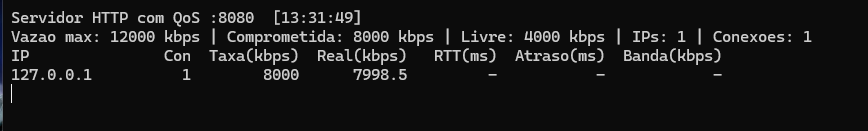
\includegraphics[width=0.82\linewidth]{painel_ip1.png}
\caption{Download de 127.0.0.1 (taxa configurada de 8000~kbps).}
\end{subfigure}\par\medskip
\begin{subfigure}{\linewidth}\centering
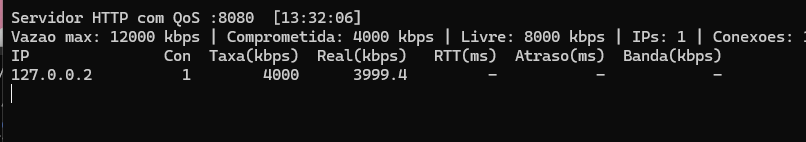
\includegraphics[width=0.82\linewidth]{painel_ip2.png}
\caption{Download de 127.0.0.2 (taxa configurada de 4000~kbps).}
\end{subfigure}
\caption{Painel do servidor durante os experimentos.}
\label{fig:painel}
\end{figure}

\subsection{Efeito do algoritmo de Nagle na medida de RTT}

Durante o desenvolvimento, a primeira medida de RTT no \textit{loopback} foi de 41,8~ms,
valor incompatível com uma comunicação local. A causa é a interação entre o algoritmo de
Nagle [Nagle 1984] e o ACK atrasado [Braden 1989]: o servidor envia o cabeçalho e o corpo
da resposta em duas chamadas \texttt{send}; com Nagle ativo, o corpo, pequeno, fica retido
até chegar o ACK do cabeçalho, e o cliente atrasa esse ACK por até cerca de 40~ms. Com
\texttt{TCP\_NODELAY} na conexão aceita, a mesma medida caiu para 0,74~ms. A mudança
também reduz o tempo de entrega de respostas pequenas e não afeta os objetos grandes, que
já são enviados em blocos completos.

\subsection{Limitações}

O \textit{loopback} não impõe as restrições de um enlace real: os experimentos verificam
a precisão do controle de taxa e da admissão implementados, mas não a variação de RTT e de
banda em uma rede física. A comparação entre clientes em rede cabeada (IEEE 802.3) e sem
fio (IEEE 802.11), com análise de capturas no Wireshark e monitoramento no IPTraf, está
prevista para a validação com o professor. No WSL2, isso exige o modo de rede espelhado,
pois a configuração padrão coloca o Linux atrás de NAT e faria todos os clientes externos
aparecerem com o mesmo endereço.

\section{Conclusões}\label{sec:concl}

A segunda versão atende aos requisitos de QoS da especificação. O relógio virtual por IP
mostrou-se uma forma simples e precisa de limitar a taxa e de dividi-la entre conexões
do mesmo endereço, com desvios abaixo de 0,7\% nos experimentos. O controle de admissão
aceitou clientes até o limite exato da vazão máxima e recusou o excedente com 503. O painel
exibe em tempo real os clientes, as taxas configurada e real e as estimativas de RTT,
atraso e banda. A investigação do RTT inflado por Nagle e ACK atrasado mostrou na prática
como decisões da camada de transporte afetam medidas feitas na camada de aplicação. Como
próximos passos, ficam os experimentos com clientes remotos em rede cabeada e sem fio, com
capturas no Wireshark e IPTraf, e a avaliação com navegadores.

\begin{thebibliography}{99}
\setlength{\itemsep}{2pt}
\makeatletter\renewcommand{\@biblabel}[1]{}\makeatother
\setlength{\leftskip}{0.5cm}\setlength{\itemindent}{-0.5cm}

\bibitem{anthropic} Anthropic (2026). \textit{Claude Code}. Ferramenta de apoio à programação utilizada na versão 2. \url{https://claude.ai/}.

\bibitem{braden} Braden, R. (1989). \textit{Requirements for Internet Hosts -- Communication Layers}. RFC 1122, IETF.

\bibitem{comer} Comer, D. E. (2016). \textit{Redes de computadores e Internet}. 6.~ed. Porto Alegre: Bookman.

\bibitem{rfc9110} Fielding, R., Nottingham, M. e Reschke, J. (2022a). \textit{HTTP Semantics}. RFC 9110, IETF.

\bibitem{rfc9112} Fielding, R., Nottingham, M. e Reschke, J. (2022b). \textit{HTTP/1.1}. RFC 9112, IETF.

\bibitem{forouzan} Forouzan, B. A. (2013). \textit{Redes de computadores: uma abordagem top-down}. Porto Alegre: AMGH.

\bibitem{kurose} Kurose, J. F. e Ross, K. W. (2013). \textit{Redes de computadores e a Internet: uma abordagem top-down}. 6.~ed. São Paulo: Pearson.

\bibitem{man} Linux man-pages project (2026). \textit{pthreads(7), clock\_nanosleep(2), tcp(7)}. \url{https://man7.org/linux/man-pages/}.

\bibitem{nagle} Nagle, J. (1984). \textit{Congestion Control in IP/TCP Internetworks}. RFC 896, IETF.

\bibitem{openai} OpenAI (2026). \textit{ChatGPT}. Ferramenta de apoio utilizada na versão 1. \url{https://chatgpt.com/}.

\bibitem{unipampa} UNIPAMPA (2026). \textit{Trabalho de Programação em Rede: especificação}. Fundamentos e Avaliação de Redes de Computadores, 2026/2.
\end{thebibliography}

\end{document}
